% Figure from MATH 591 notes, section 16. Compile with the notes preamble.
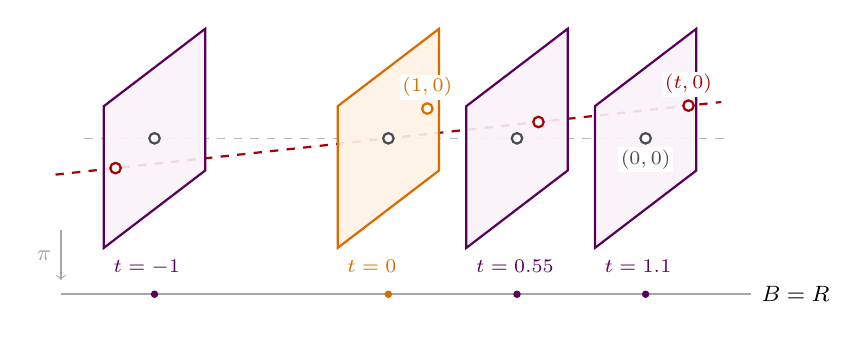
\begin{tikzpicture}[scale=0.9]
\draw[gray!55, dashed] (-4.290,0.000) -- (4.785,0.000);
\draw[red!65!black, dashed, thick] (-4.697,-0.512) -- (4.697,0.512);
\draw[violet!70!black, thick, fill=violet!5, fill opacity=0.9] (-4.015,-1.546) -- (-2.585,-0.454) -- (-2.585,1.546) -- (-4.015,0.454) -- cycle;
\draw[gray!60!black, fill=white, thick] (-3.300,0.000) circle (2.1pt);
\draw[red!65!black, fill=white, thick] (-3.850,-0.420) circle (2.1pt);
\node[font=\scriptsize, text=violet!70!black, anchor=north west] at (-4.015,-1.586) {$t = -1$};
\draw[orange!85!black, thick, fill=orange!10, fill opacity=0.9] (-0.715,-1.546) -- (0.715,-0.454) -- (0.715,1.546) -- (-0.715,0.454) -- cycle;
\draw[gray!60!black, fill=white, thick] (0.000,0.000) circle (2.1pt);
\draw[orange!85!black, fill=white, thick] (0.550,0.420) circle (2.1pt);
\node[font=\scriptsize, text=orange!85!black, anchor=north west] at (-0.715,-1.586) {$t = 0$};
\draw[violet!70!black, thick, fill=violet!5, fill opacity=0.9] (1.100,-1.546) -- (2.530,-0.454) -- (2.530,1.546) -- (1.100,0.454) -- cycle;
\draw[gray!60!black, fill=white, thick] (1.815,0.000) circle (2.1pt);
\draw[red!65!black, fill=white, thick] (2.118,0.231) circle (2.1pt);
\node[font=\scriptsize, text=violet!70!black, anchor=north west] at (1.100,-1.586) {$t = 0.55$};
\draw[violet!70!black, thick, fill=violet!5, fill opacity=0.9] (2.915,-1.546) -- (4.345,-0.454) -- (4.345,1.546) -- (2.915,0.454) -- cycle;
\draw[gray!60!black, fill=white, thick] (3.630,0.000) circle (2.1pt);
\draw[red!65!black, fill=white, thick] (4.235,0.462) circle (2.1pt);
\node[font=\scriptsize, text=violet!70!black, anchor=north west] at (2.915,-1.586) {$t = 1.1$};
\node[orange!85!black, font=\scriptsize, anchor=south, fill=white, inner sep=1pt] at (0.550,0.540) {$(1,0)$};
\node[red!65!black, font=\scriptsize, anchor=south, fill=white, inner sep=1pt] at (4.235,0.582) {$(t,0)$};
\node[gray!60!black, font=\scriptsize, anchor=north, fill=white, inner sep=1pt] at (3.630,-0.120) {$(0,0)$};
\draw[thick, gray!70] (-4.62,-2.2) -- (5.12,-2.2) node[right, font=\footnotesize, text=black] {$B = \mathbb{R}$};
\fill[violet!70!black] (-3.300,-2.2) circle (1.5pt);
\fill[orange!85!black] (0.000,-2.2) circle (1.5pt);
\fill[violet!70!black] (1.815,-2.2) circle (1.5pt);
\fill[violet!70!black] (3.630,-2.2) circle (1.5pt);
\draw[->, gray!70] (-4.62,-1.3) -- node[left, font=\footnotesize] {$\pi$} (-4.62,-2.0);
\end{tikzpicture}
